\documentclass[11pt]{article}

\usepackage[margin=1in]{geometry}
\usepackage{booktabs}
\usepackage{graphicx}
\usepackage{amsmath}
\usepackage{amssymb}
\usepackage{hyperref}
\usepackage{array}
\usepackage{xcolor}

\title{Citation Faithfulness in Open-Weight Retrieval-Augmented Generation}
\author{Abimbola Jeremiah}
\date{August 2026}

\begin{document}
\sloppy
\maketitle

\begin{abstract}
Retrieval-augmented generation (RAG) systems often present citations as evidence that an answer is grounded in retrieved documents. A citation can be correct in the weak sense that the cited text agrees with the answer, while still being unfaithful if the model would have produced the same answer from parametric memory and attached the citation after the fact. We study this distinction in three open-weight instruction-tuned models: Llama-3.1-8B-Instruct, Qwen2.5-7B-Instruct, and Gemma-3-12B-it. The experiment combines a Natural Questions and KILT Wikipedia behavioral post-rationalization benchmark, a ConflictBank counterfactual validation set, a Llama-only activation-patching analysis on PopQA capital questions, and linear probes trained on hidden states to predict post-rationalized citations. Across models, random forged documents rarely receive citations, while forged documents with stronger apparent relevance are cited more often. Qwen shows the highest post-rationalization rate in the cited-other condition (21.6\%), followed by Gemma (17.8\%) and Llama (9.1\%). ConflictBank results show a strong preference for supplied context even under conflict. Linear probes recover the behavioral label above simple lexical and semantic baselines, with AUROC values of 0.943 for Llama, 0.969 for Qwen, and 0.831 for Gemma. The mechanistic intervention validation did not produce successful causal edits in this run, suggesting that the selected components were insufficient for robustly controlling citation behavior on generated text. Together, the results support the view that citation faithfulness is distinct from citation correctness and can be measured behaviorally and partially decoded from internal representations.
\end{abstract}

\section{Introduction}

Retrieval-augmented generation (RAG) combines parametric language models with retrieved documents to improve performance on knowledge-intensive tasks \cite{lewis2020rag,guu2020realm,izacard2021fid}. In practical RAG systems, citations are the interface between an answer and its purported evidence. They allow readers to inspect the source of a claim and are commonly treated as signals that the cited material supported generation. This expectation is especially consequential in information-seeking settings, where users may rely on citations to judge whether an answer is verifiable \cite{liu2023verifiability}.

The apparent transparency of a cited answer can conceal several distinct operations. A retriever selects documents, a generator produces a claim while attending to those documents and its parametric knowledge, and the system emits a citation marker that links the claim to one of the retrieved sources. Success at the final operation does not guarantee success at the others. A system may retrieve a relevant passage but ignore it, generate a memorized answer, and then select a textually compatible citation. The resulting output can look well grounded to a reader even though the citation is not an accurate account of how the answer was produced. This gap matters because citations are not merely an output format: they are often used as a practical proxy for provenance, auditability, and appropriate reliance on external evidence.

Generating citations is not equivalent to establishing that they faithfully reflect model behavior. Attributed-generation systems have made substantial progress on producing answers with citations and evaluating whether cited passages entail individual claims \cite{gao2023citations}. These evaluations primarily measure citation correctness or completeness: whether a passage supports a claim and whether claims receive support. They do not, by themselves, determine whether a model used that passage rather than parametric knowledge or a superficial document-answer match. A citation can therefore be correct in content while failing as an explanation of the model's actual evidence use.

We use \emph{citation correctness} for the textual relation between a claim and a cited passage, and \emph{citation faithfulness} for the relation between the citation and the model's evidence use during generation. The distinction is causal rather than stylistic. Correctness can be evaluated from the completed answer and passage, whereas faithfulness requires asking how the output changes when the evidential role of a document changes. No single observable fully resolves that question: behavioral interventions can expose sensitivity to forged support, activation patching can test narrowly specified internal mechanisms, and probes can reveal whether a risk label is encoded in hidden states. These forms of evidence answer different questions and should not be treated as interchangeable.

Wallat et al. formalize this distinction for RAG attributions and introduce post-rationalization interventions, in which an answer-bearing string is inserted into a document that does not provide the original factual support \cite{wallat2025correctness}. If a model recovers the target statement and cites that document, the result challenges an interpretation of the citation as provenance. This concern is complementary to work that derives attributions from model internals, such as context-sensitive token analysis and saliency-based document attribution \cite{qi2024mirage}. Together, these lines of work motivate evaluations that distinguish textual support from causal reliance on retrieved context.

Open-weight instruction-tuned models provide a useful setting for such an evaluation. They support controlled generation experiments across model families while also exposing the hidden states and intermediate activations needed for representation-level and causal analyses. This makes it possible to compare what models do under document interventions, what information their representations contain, and whether selected internal components can control citation behavior. At the same time, access to activations does not make faithfulness directly observable. A successful probe establishes predictability, and a successful patch establishes a causal effect under a particular intervention; neither alone proves that a generated citation is a complete explanation of the model's reasoning.

We organize the study around three questions. First, how often will a model cite an adversarial document when that document contains an answer-bearing phrase but lacks the original evidential role, and how does this behavior change as the forged document becomes more contextually plausible? Second, does citation post-rationalization leave a linearly decodable signal in model hidden states beyond lexical and semantic similarity cues? Third, can activation patching identify components whose manipulation reliably changes citation behavior during full generation? A counterfactual knowledge-conflict experiment provides an additional view of how strongly each model follows supplied context when it disagrees with parametric knowledge.

This paper studies citation faithfulness in three open-weight instruction-tuned RAG models: Llama-3.1-8B-Instruct, Qwen2.5-7B-Instruct, and Gemma-3-12B-it. We make four contributions. First, we measure behavioral post-rationalization on Natural Questions with KILT Wikipedia retrieval under random, relevant-uncited, and cited-other document interventions. Second, we use ConflictBank to characterize model behavior when supplied context conflicts with parametric knowledge. Third, we test a narrow causal hypothesis about citation behavior in Llama-3.1-8B-Instruct through activation patching on PopQA capital-city examples. Fourth, we evaluate whether post-rationalization labels are linearly decodable from hidden states and whether these probes improve on lexical, logit-margin, and embedding-similarity baselines. The resulting evidence separates behavioral, causal, and predictive perspectives on citation faithfulness without conflating any one of them with citation correctness.

The results show a consistent but conditional vulnerability. Random forged documents are almost never cited, but citation rates rise when the adversarial document is topically relevant or has already appeared elsewhere in the model's citation context. The cited-other condition produces post-rationalization rates of 9.1\% for Llama, 21.6\% for Qwen, and 17.8\% for Gemma, while ConflictBank shows that all three models strongly prefer supplied context under conflict. Hidden-state probes predict the behavioral label substantially better than the evaluated baselines, indicating that post-rationalization risk is represented beyond simple surface matching. By contrast, the selected Llama components do not yield successful generation-level edits in our mechanistic validation. The combined picture is therefore neither that citations are arbitrary nor that textual support guarantees provenance: citation faithfulness is behaviorally measurable and predictively encoded, but robust causal control remains unresolved in this experimental setting.

\section{Related Work}

Early RAG architectures coupled parametric language models with external retrieval for knowledge-intensive tasks. REALM integrates retrieval into language-model pre-training, RAG marginalizes over retrieved passages during generation, and Fusion-in-Decoder aggregates evidence from multiple passages in the decoder \cite{guu2020realm,lewis2020rag,izacard2021fid}. These systems established that retrieval can improve factual and open-domain question answering, but their standard outcome measures primarily concern answer quality. Natural Questions provides naturally occurring information-seeking queries with annotated answers, while KILT unifies knowledge-intensive tasks around a shared Wikipedia snapshot and provenance annotations \cite{kwiatkowski2019natural,petroni2021kilt}. Such resources make retrieval and answer provenance evaluable, yet a relevant retrieved passage and a correct answer do not show that the generator relied on that passage for a particular claim. Our use of Natural Questions and KILT therefore begins from established retrieval evaluation but changes the target from answer accuracy to the behavior of generated citations under controlled document interventions.

Attributed generation makes provenance visible by requiring systems to accompany generated claims with source references. Gao et al. compare inline and post-hoc citation generation and evaluate citation quality through entailment and completeness at the claim level \cite{gao2023citations}. Liu et al. study generative search engines from the reader's perspective, measuring whether claims are supported by citations and whether those citations enable verification \cite{liu2023verifiability}. This work supplies important criteria for useful citations: claims should be covered, cited sources should support them, and references should be inspectable. These criteria evaluate the relationship between the final claim and source, however, rather than the source's role in producing the claim. A model can generate a memorized fact and subsequently attach an entailing passage, satisfying a correctness criterion while giving a potentially misleading account of provenance. Our study treats citation correctness as necessary for trustworthy attributed generation but not sufficient for citation faithfulness.

Citation faithfulness asks whether an emitted attribution reflects the evidence that influenced generation. Wallat et al. formalize the distinction between correctness and faithfulness in RAG and introduce adversarial interventions that place answer-bearing strings in documents lacking the original evidential role \cite{wallat2025correctness}. Citation of such a document after recovery of the target statement provides behavioral evidence of post-rationalization. Qi et al. pursue faithful answer attribution from model internals, combining context sensitivity and saliency to estimate which retrieved documents affect answer tokens \cite{qi2024mirage}. The two approaches differ in observability and scope: adversarial tests expose behavior under controlled input changes, whereas internal attribution methods estimate influence within a particular forward computation. We extend the intervention-based approach across three open-weight model families and three levels of adversarial plausibility, then connect its behavioral labels to internal representations without treating decodability as proof of causal reliance.

The distinction between retrieved evidence and parametric memory is also central to work on knowledge conflicts. PopQA examines when language models succeed from parametric memory and when non-parametric evidence is beneficial, with entity popularity providing an important source of variation \cite{mallen2023popqa}. ConflictBank directly evaluates cases in which supplied context conflicts with a model's parametric knowledge and measures which source dominates the response \cite{su2024conflictbank}. Conflict following is related to, but distinct from, citation faithfulness. A context-matching answer demonstrates sensitivity to supplied evidence, while a faithful citation additionally requires that the cited document accurately identify the evidence used for the associated claim. We use ConflictBank as secondary counterfactual validation and reserve PopQA capital relations for the mechanistic analysis; neither dataset is used to define the behavioral post-rationalization labels.

Mechanistic interpretability offers tools for moving from input-output association to localized causal hypotheses. Causal tracing and activation editing have identified transformer components involved in recalling factual associations and shown that intervening on internal states can alter model predictions \cite{meng2022rome}. TransformerLens provides hooks and activation-caching abstractions commonly used for such patching experiments \cite{nanda2022transformerlens}. Most directly, van Dort and Heuss study citation generation in Llama-3.1-8B-Instruct through activation patching on PopQA and a citation-token logit-difference metric \cite{vandort2026cite}. We adapt this design to a restricted capital-city subset, distinguish component discovery from downstream validation, and test whether components selected by token-level patching can control citations during autoregressive generation.

Linear probes address a different question: whether a target property is recoverable from a model representation by a simple classifier. Strong probe performance can demonstrate that information associated with a label is linearly available, but it does not establish that the model uses that information or that the probed direction causes the behavior \cite{belinkov2022probes}. Accordingly, our layer-wise probes are evaluated as predictors of intervention-derived post-rationalization labels and compared with lexical overlap, citation-logit, and semantic-similarity baselines. The behavioral interventions, mechanistic patches, and probes thus form complementary evidence: they test observable vulnerability, a narrow causal mechanism, and internal predictability, respectively.

\section{Methodology}

\subsection{Research Architecture}

Figure~\ref{fig:research-architecture} summarizes the experimental architecture. The primary pipeline starts from Natural Questions, KILT Wikipedia, and ConflictBank inputs; retrieves top-$5$ BM25 contexts from 100-token Wikipedia chunks; runs deterministic generation with the three open-weight instruction-tuned models; applies behavioral interventions; and evaluates post-rationalization through citation labels and hidden-state probes. A separate auxiliary mechanistic path uses PopQA capital-city pairs for Llama-only activation patching, component selection, and generation-level validation. This separation keeps the behavioral comparison across all models distinct from the narrower causal analysis performed on Llama.

\begin{figure*}[t]
\centering
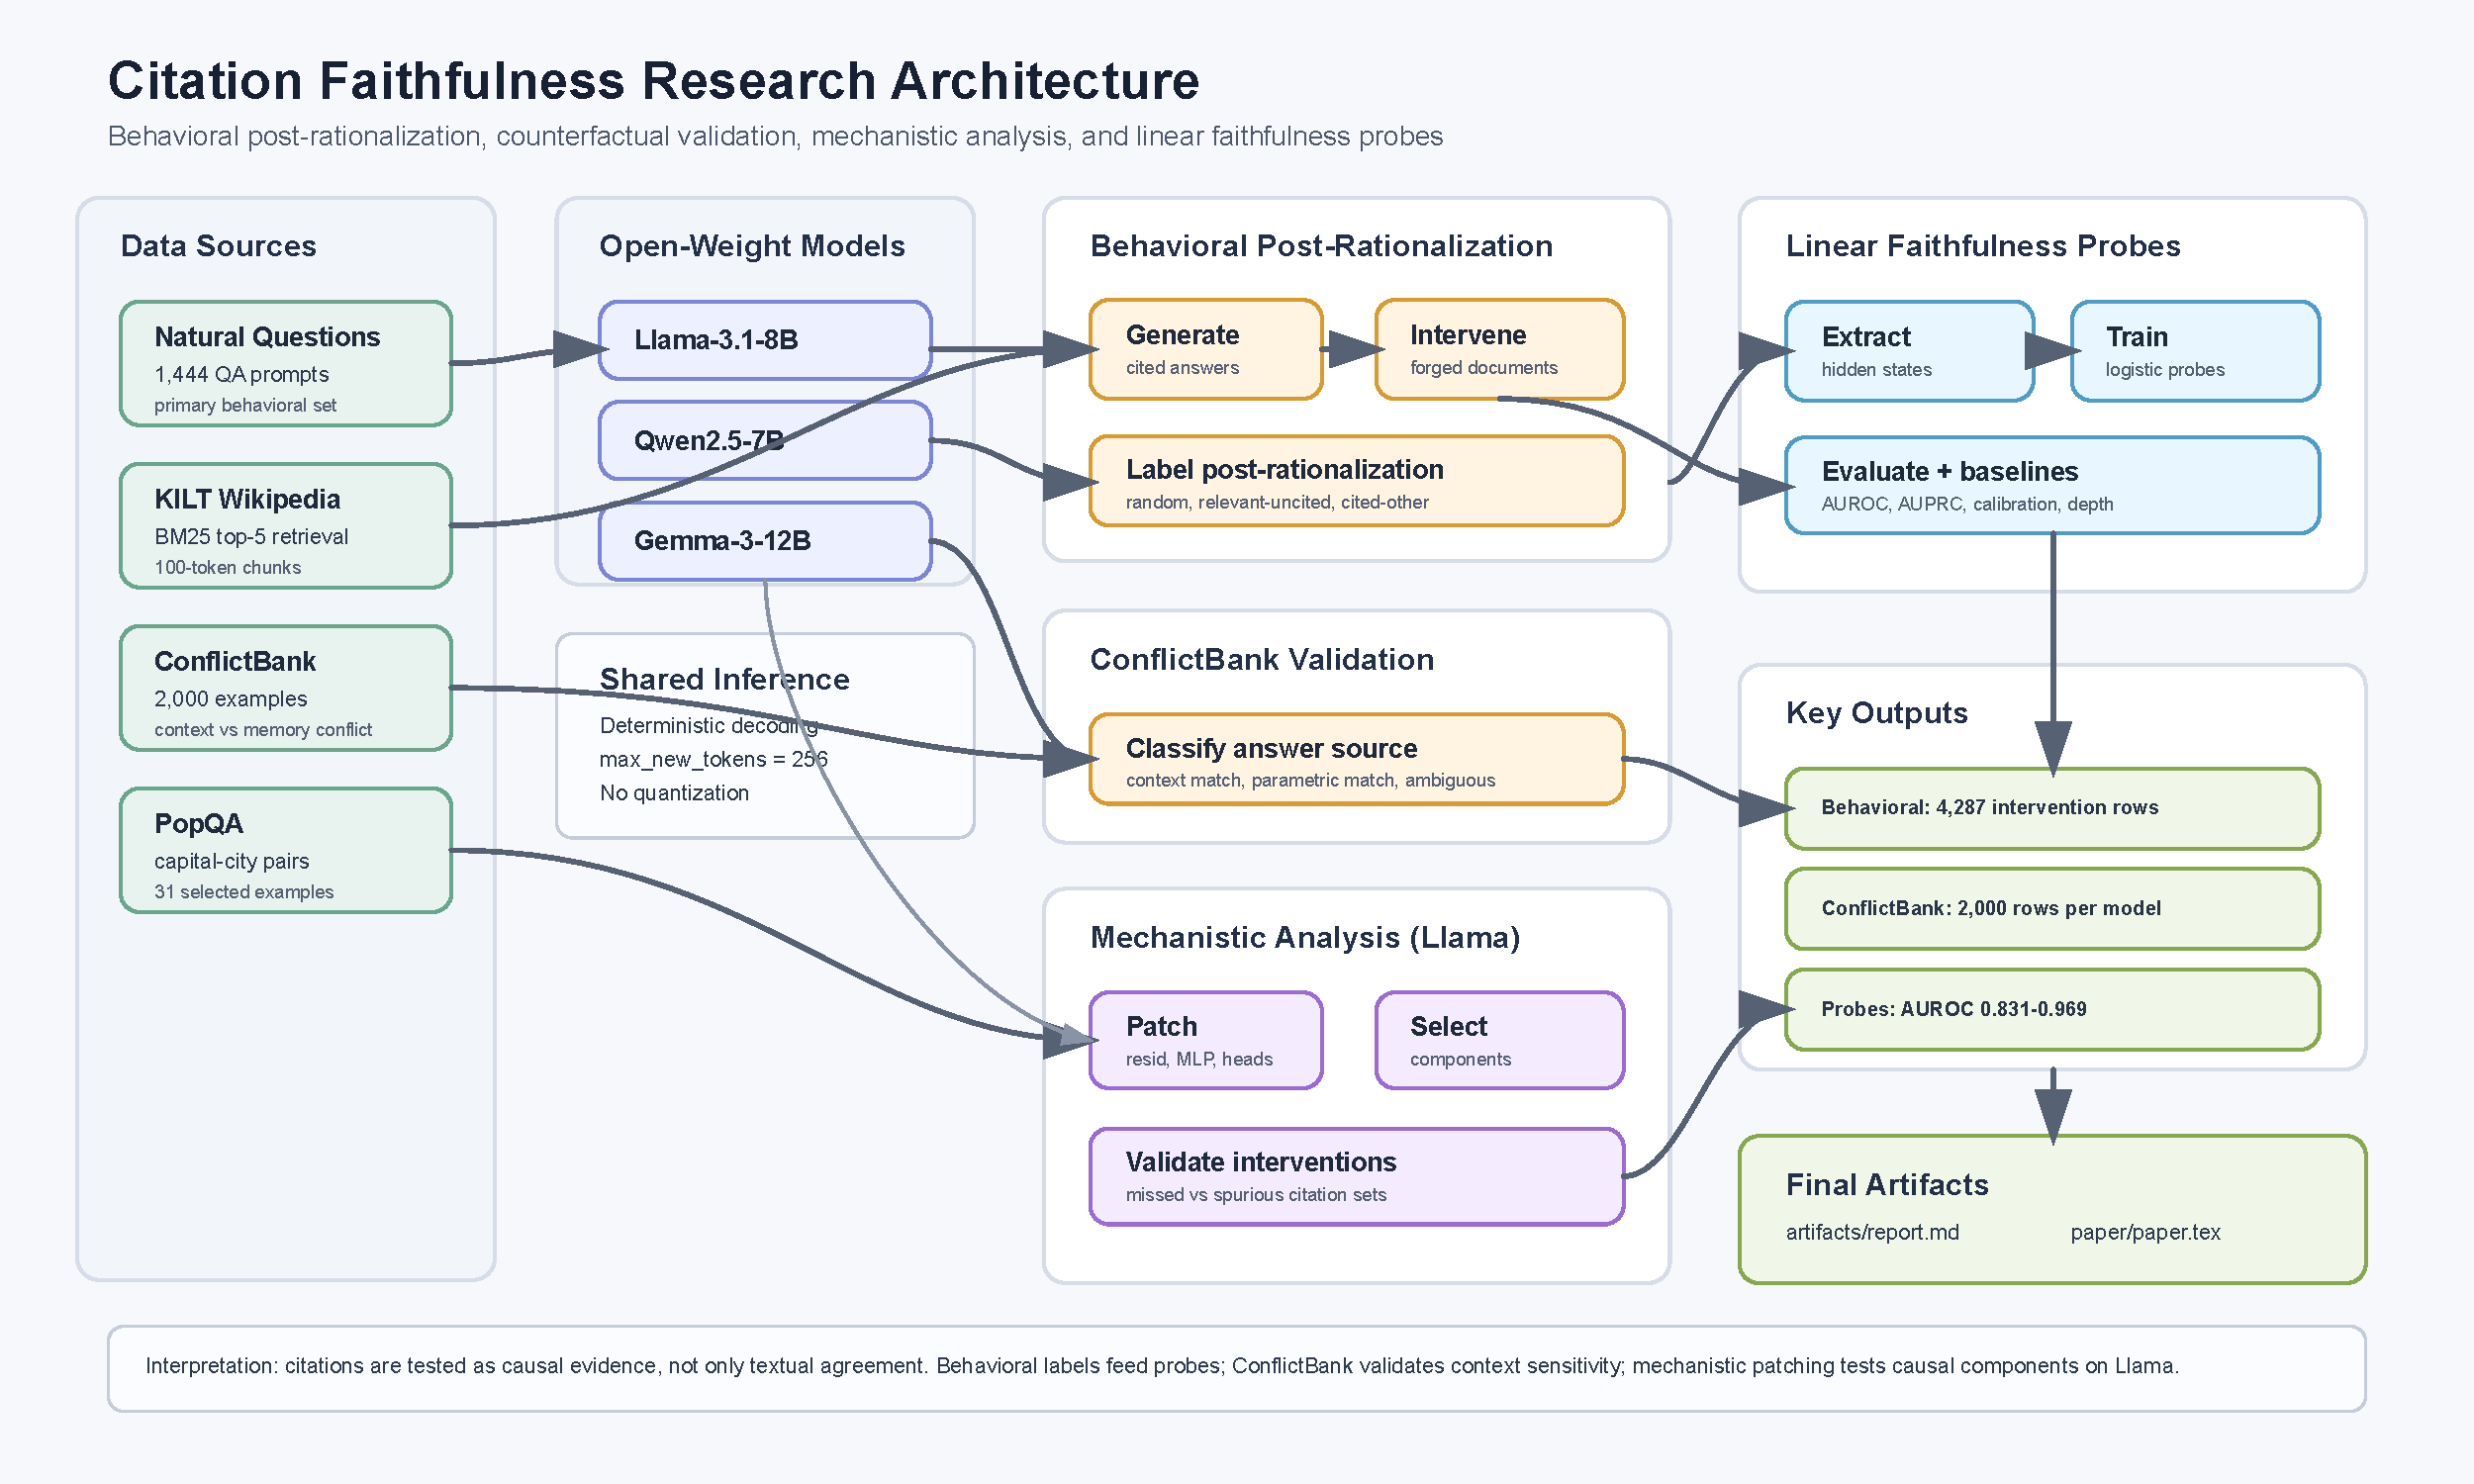
\includegraphics[width=\textwidth]{figures/research_architecture.pdf}
\caption{Research architecture for the citation-faithfulness experiments. The main path evaluates retrieval, generation, behavioral interventions, and probes across all three models; the auxiliary mechanistic path performs Llama-only activation patching on PopQA examples.}
\label{fig:research-architecture}
\end{figure*}

\subsection{Models and Data}

All model weights and tokenizers were obtained from their official Hugging Face releases. We used the instruction-tuned checkpoints \href{https://huggingface.co/meta-llama/Llama-3.1-8B-Instruct}{\texttt{meta-llama/Llama-3.1-8B-Instruct}}, \href{https://huggingface.co/Qwen/Qwen2.5-7B-Instruct}{\texttt{Qwen/Qwen2.5-7B-Instruct}}, and \href{https://huggingface.co/google/gemma-3-12b-it}{\texttt{google/gemma-3-12b-it}}, developed by Meta, Alibaba's Qwen team, and Google DeepMind, respectively \cite{grattafiori2024llama3,yang2024qwen25,gemmateam2025gemma3}. Llama 3.1 and Gemma 3 require acceptance of their respective model licenses, while Qwen2.5 is distributed under the Apache 2.0 license. These open-weight checkpoints permit hidden-state extraction and activation patching in addition to generation. The semantic-similarity baseline used \href{https://huggingface.co/sentence-transformers/all-mpnet-base-v2}{\texttt{sentence-transformers/all-mpnet-base-v2}} to encode document-query pairs, following the sentence-transformer bi-encoder approach \cite{reimers2019sentencebert}.

The behavioral question set comprised the 1,444 unique Natural Questions identifiers and questions released with the experiments of Wallat et al. \cite{wallat2025correctness}; the underlying questions originate from Natural Questions \cite{kwiatkowski2019natural}. Retrieved evidence came from the full KILT Wikipedia knowledge source \cite{petroni2021kilt}. The full Wikipedia pages were converted to non-overlapping 100-whitespace-token chunks before BM25 retrieval. Thus, the Natural Questions release supplied the query set, while KILT supplied the document corpus.

The mechanistic examples were obtained from the \href{https://huggingface.co/datasets/akariasai/PopQA}{\texttt{akariasai/PopQA}} test split \cite{mallen2023popqa}. We retained capital-city relations and constructed the clean and corrupted pairs described below. The counterfactual validation data were obtained from the \href{https://huggingface.co/datasets/Warrieryes/CB_qa}{\texttt{Warrieryes/CB\_qa}} training split associated with ConflictBank \cite{su2024conflictbank}; the experiment streamed that split, retained the first 2,000 schema-valid examples, and sorted them by example identifier before generation. ConflictBank was used only for secondary validation, and PopQA was used only for mechanistic analysis. Probe labels and features were derived from our own behavioral interventions rather than imported from either dataset.

\subsection{Models and Execution}

We evaluated three open-weight instruction-tuned models: \texttt{meta-llama/Llama-3.1-8B-Instruct}, \texttt{Qwen/Qwen2.5-7B-Instruct}, and \texttt{google/gemma-3-12b-it}. Behavioral and probe experiments were run for all three models. Mechanistic activation patching was run only for Llama-3.1-8B-Instruct, matching the mechanistic scope of the study. Generation used deterministic greedy decoding with a maximum of 256 new tokens. The experiments used Apple MPS with backend-selected reduced precision and no quantization.

\subsection{Behavioral Post-Rationalization Benchmark}

The primary behavioral benchmark uses 1,444 Natural Questions queries and KILT Wikipedia retrieval with top-$5$ BM25 contexts. For each model, we first generated answers with citations under a system instruction requiring citation of document-supported claims. We then parsed cited statements and constructed interventions around target statements that the model originally cited.

Each target statement was tested under three adversarial conditions:

\begin{itemize}
    \item \textbf{Random}: the answer-bearing phrase is inserted into an otherwise random document, placed at citation index $[5]$.
    \item \textbf{Relevant uncited}: the phrase is inserted into a retrieved document that is topically relevant but was not the original cited source.
    \item \textbf{Cited other}: the phrase is inserted into another document that the model cited elsewhere in the original answer.
\end{itemize}

An intervention is counted as available when the adversarial document can be constructed. The model output is labeled \textsc{post-rationalized} when the target statement is recovered and the adversarial document's citation marker appears in the sentence containing the recovered target phrase. The main metric is therefore the adversarial citation rate conditional on statement recovery and condition availability:

\begin{equation}
    \mathrm{PRR} = \frac{\#\{\mathrm{recovered\ target\ and\ adversarial\ citation}\}}{\#\{\mathrm{condition\ available\ and\ recovered\ target}\}}.
\end{equation}

Wilson 95\% intervals were computed for the conditional rate.

\subsection{ConflictBank Validation}

ConflictBank is used as a secondary validation experiment rather than as probe training data. Each model answered 2,000 conflict examples. The setup tests whether the model's answer aligns with supplied conflicting evidence, parametric knowledge, or neither. We report the resulting label-transition counts and the overall rate of context-matching predictions.

\subsection{Mechanistic Activation Patching}

For mechanistic analysis, we constructed capital-city pairs from PopQA \cite{mallen2023popqa}. A clean prompt contains a document of the form ``$A$ is the capital of $S$'' and asks the corresponding question. A corrupted prompt replaces the clean document with a distractor document whose tokenization is length-matched for subject and answer spans. We selected the first 31 examples for which the citation logit difference is positive in the clean prompt and negative in the corrupted prompt:

\begin{equation}
    \Delta = \mathrm{logit}(\texttt{" ["}) - \mathrm{logit}(\texttt{"."}).
\end{equation}

For each selected example, we cached clean and corrupted activations and patched residual streams, MLP outputs, and attention heads. Denoising recovery and noising degradation were computed as

\begin{equation}
    R_{\mathrm{denoise}} = \frac{\Delta_{\mathrm{patched}} - \Delta_{\mathrm{corrupt}}}{\Delta_{\mathrm{clean}} - \Delta_{\mathrm{corrupt}}},
    \quad
    D_{\mathrm{noise}} = \frac{\Delta_{\mathrm{clean}} - \Delta_{\mathrm{patched}}}{\Delta_{\mathrm{clean}} - \Delta_{\mathrm{corrupt}}}.
\end{equation}

Components were selected as positive if mean denoising recovery was at least 0.10 and necessary if mean noising degradation was at least 0.20. The selected components were then tested by scaling them during generation on missed-citation and spurious-citation examples.

\subsection{Linear Faithfulness Probes}

For each model, we extracted hidden-state features from behavioral intervention examples labeled \textsc{post-rationalized} or \textsc{not-post-rationalized}. The decision position was the first adversarial citation marker when present; otherwise it was the sentence position associated with the target phrase. For each layer, the feature vector was the mean hidden state over the decision token and the two preceding answer tokens.

Questions were split by \texttt{question\_id} into 70\% train, 15\% validation, and 15\% test partitions to avoid leakage across interventions for the same question. We trained one L2 logistic regression probe per layer with balanced class weights, selected the layer with best validation AUROC, and reported test AUROC, AUPRC, balanced accuracy, F1, and Brier score. Baselines used lexical overlap, citation-logit margin, and document-query cosine similarity from a sentence-transformer encoder.

\section{Experimental Results}

\subsection{Behavioral Post-Rationalization}

Table~\ref{tab:behavioral} reports conditional post-rationalization rates. Random forged documents are rarely cited. Rates increase for relevant-uncited and cited-other documents, suggesting that stronger topical or citation-context cues make shallow attribution more likely.

\begin{table*}[t]
\centering
\small
\begin{tabular}{llrrrr}
\toprule
Model & Condition & Post-rationalized & Available & Rate & Wilson 95\% CI \\
\midrule
Llama-3.1-8B & Random & 0 & 274 & 0.0\% & [0.0, 1.7] \\
Llama-3.1-8B & Relevant uncited & 8 & 245 & 3.5\% & [1.8, 6.7] \\
Llama-3.1-8B & Cited other & 2 & 23 & 9.1\% & [2.5, 27.8] \\
Qwen2.5-7B & Random & 3 & 326 & 1.1\% & [0.4, 3.2] \\
Qwen2.5-7B & Relevant uncited & 27 & 299 & 9.7\% & [6.7, 13.7] \\
Qwen2.5-7B & Cited other & 11 & 59 & 21.6\% & [12.5, 34.6] \\
Gemma-3-12B & Random & 4 & 829 & 0.6\% & [0.2, 1.5] \\
Gemma-3-12B & Relevant uncited & 13 & 726 & 1.9\% & [1.1, 3.2] \\
Gemma-3-12B & Cited other & 18 & 117 & 17.8\% & [11.6, 26.4] \\
\bottomrule
\end{tabular}
\caption{Behavioral post-rationalization rates conditional on condition availability and target statement recovery.}
\label{tab:behavioral}
\end{table*}

The pattern is consistent across the three model families. The random condition acts as a low-rate control. The cited-other condition is most adversarial because the document is already plausible in the model's citation context; Qwen and Gemma show substantial vulnerability in this condition. Llama is more conservative, but the cited-other condition has low availability for Llama, so the confidence interval is wide.

\subsection{ConflictBank}

Table~\ref{tab:conflictbank} summarizes ConflictBank outcomes. All models predict context-matching answers for more than 80\% of the 2,000 examples, despite the benchmark being designed around conflict. This supports the behavioral finding that the supplied context exerts strong pressure on answer and citation behavior.

\begin{table}[t]
\centering
\small
\begin{tabular}{lrrrr}
\toprule
Model & Total & Context match & Parametric match & Ambiguous \\
\midrule
Llama-3.1-8B & 2000 & 1657 (82.9\%) & 28 (1.4\%) & 315 (15.8\%) \\
Qwen2.5-7B & 2000 & 1710 (85.5\%) & 24 (1.2\%) & 266 (13.3\%) \\
Gemma-3-12B & 2000 & 1680 (84.0\%) & 22 (1.1\%) & 298 (14.9\%) \\
\bottomrule
\end{tabular}
\caption{ConflictBank prediction distribution aggregated over 2,000 examples per model.}
\label{tab:conflictbank}
\end{table}

\subsection{Mechanistic Patching and Interventions}

The PopQA mechanistic phase selected 31 qualifying clean/corrupted pairs. Patching produced 512 residual entries, 512 MLP entries, and 1,024 attention-head entries. Component selection found no positive citation heads or MLP components under the denoising threshold. It identified one necessary head, layer 0 head 3, and 11 necessary MLP positions in layer 0.

Validation found 7 missed-citation examples and 58 spurious-citation examples, but component scaling did not successfully fix either class: both success rates were 0.0. This negative result should be interpreted carefully. Activation patching showed early components with a measurable causal effect on the citation logit difference, but the simple intervention of uniformly scaling selected components was not sufficient to control full autoregressive generation.

\begin{table}[t]
\centering
\small
\begin{tabular}{lrr}
\toprule
Validation set & Count & Success rate \\
\midrule
Missed citation & 7 & 0.0\% \\
Spurious citation & 58 & 0.0\% \\
\bottomrule
\end{tabular}
\caption{Mechanistic intervention validation after component selection and scaling.}
\label{tab:mechanistic-validation}
\end{table}

\subsection{Faithfulness Probes}

The probe datasets contained 15,328 Llama feature rows, 16,912 Qwen feature rows, and 70,272 Gemma feature rows. Table~\ref{tab:probes} reports held-out test performance for the selected layer of each model. The selected layers cluster around 60--68\% relative depth, consistent with the idea that the behavioral faithfulness signal is most linearly available in middle-to-late residual streams.

\begin{table*}[t]
\centering
\small
\begin{tabular}{lrrrrrr}
\toprule
Model & Layer & Rel. depth & AUROC & AUPRC & Bal. acc. & Best baseline AUROC \\
\midrule
Llama-3.1-8B & 21 & 0.68 & 0.943 & 0.200 & 0.479 & 0.757 \\
Qwen2.5-7B & 17 & 0.63 & 0.969 & 0.325 & 0.918 & 0.908 \\
Gemma-3-12B & 28 & 0.60 & 0.831 & 0.357 & 0.616 & 0.716 \\
\bottomrule
\end{tabular}
\caption{Test performance of selected-layer linear probes. Best baseline AUROC is the maximum over lexical overlap, citation-logit margin, and document-query cosine similarity.}
\label{tab:probes}
\end{table*}

The probes outperform the strongest simple baseline by AUROC for all three models. Qwen is the clearest case, with both high ranking performance and high balanced accuracy. Llama has high AUROC but low F1 and balanced accuracy at the default 0.5 threshold, reflecting the very small number of positive test examples. Gemma has weaker AUROC than Llama and Qwen but the highest AUPRC among the three, again under substantial label imbalance.

\section{Discussion}

The behavioral results support a graded picture of citation faithfulness. The models do not blindly cite arbitrary forged documents. However, they become more likely to cite adversarial documents when those documents are topically relevant or already citation-plausible. This suggests that citation selection is sensitive to document-answer compatibility signals that are weaker than genuine provenance.

The ConflictBank results point in the same direction from a different angle. When supplied evidence conflicts with parametric knowledge, all three models usually align with the supplied context. This is desirable when the context is correct, but it also means that document placement and surface evidence can strongly steer answers.

The mechanistic results are more mixed. Activation patching identifies early necessary components, but the downstream scaling intervention does not produce successful behavioral control. One interpretation is that the citation decision is distributed and context-sensitive: components that affect a next-token citation logit under controlled prompts may not be sufficient to control multi-token answer generation. Another possibility is that the local MPS precision and the simple scaling intervention make the validation underpowered. Either way, the negative validation is a useful constraint on mechanistic claims.

The probe results are practically promising. Even with simple logistic regression and no learned neural probe architecture, the hidden states contain a linearly decodable signal predictive of post-rationalization. This does not prove that the selected feature is causally responsible for unfaithful citation behavior. It does suggest that faithfulness risk could be monitored without rerunning the full adversarial intervention for every generation.

\section{Limitations}

This study uses a specific operational definition of citation faithfulness. It detects post-rationalization under answer-string insertion interventions, not every possible form of unfaithful attribution. The Natural Questions setup depends on BM25 retrieval over KILT Wikipedia chunks and on parser heuristics for cited statements. The cited-other condition has low availability for Llama, leading to wide confidence intervals. The mechanistic experiment is intentionally narrow: Llama only, PopQA capital facts only, and citation-token-versus-period logit difference as the target. The probe labels are imbalanced, especially for Llama and Gemma, so AUROC is more stable than F1. Finally, the local run used Apple MPS rather than CUDA, so exact numerical reproduction may differ on the original CUDA-oriented setup.

\section{Conclusion}

The experiment shows that citation faithfulness is not guaranteed by citation correctness in open-weight RAG models. Across Llama, Qwen, and Gemma, adversarial documents containing answer-bearing strings can attract citations, especially when the document is topically or citation-context plausible. ConflictBank confirms that supplied context strongly influences model outputs under conflict. Mechanistic patching identifies early Llama components associated with citation-logit behavior, but simple component scaling does not yield successful generation-level interventions. Linear probes, however, predict post-rationalization labels above simple baselines, indicating that faithfulness-relevant information is present in internal states. A practical next step is to improve intervention methods and calibrate probes as runtime monitors for citation faithfulness risk.

\bibliographystyle{plain}
\bibliography{references}

\end{document}
